%!TEX root = ../dokumentation.tex

\chapter{Bedienung der Anwendung}
\begin{wrapfigure}{r}{120px}
\label{Bild1}
\centering
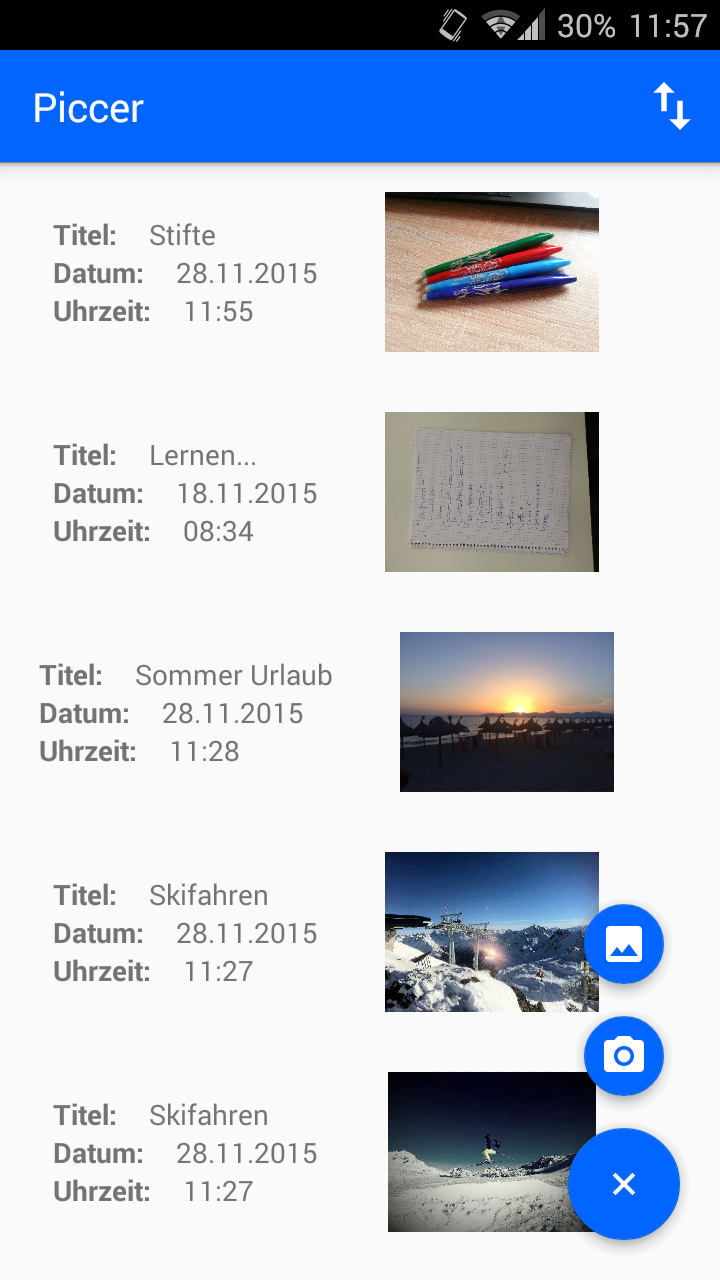
\includegraphics[width=120px]{../images/bild_1}
\caption{Übersicht}
\end{wrapfigure}
Abbildung \ref{Bild1} zeigt die Anwendung nach dem Start. Zu sehen ist eine Liste von Bildern, die der App entweder durch das Aufnehmen eines Fotos oder das Laden eines Bildes
aus der Galerie, hinzugefügt wurde. Links neben dem Foto werden ein Titel, das Datum und die Uhrzeit, an dem das Bild aufgenommen wurde, angezeigt. \\
Wird ein Bild aus der Galerie geladen und es liegt ein Datum vor, als das Bild erstellt wurde, so zeigt \enquote{Piccer} dieses Datum an. Falls es nicht möglich ist, ein solches
\begin{wrapfigure}{r}{120px}
\label{Bild2}
\centering
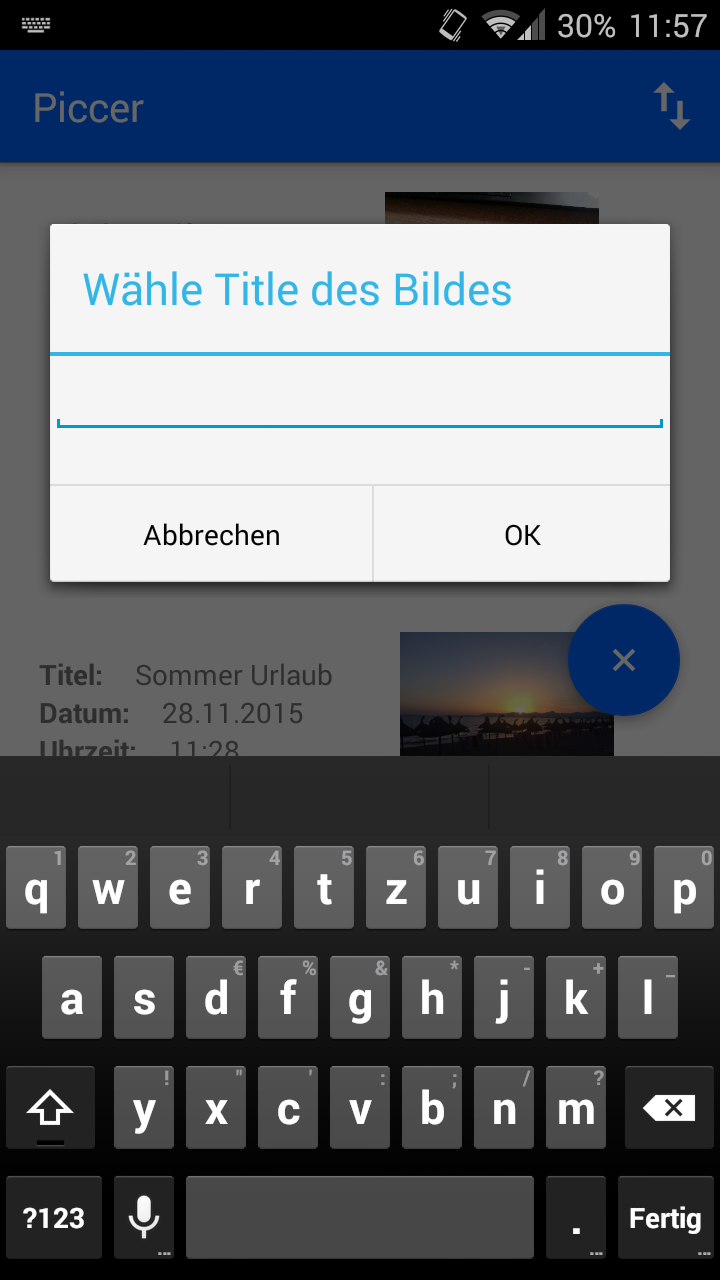
\includegraphics[width=120px]{../images/bild_2}
\caption{Titel vergeben}
\end{wrapfigure}
Datum aus der Datei auszulesen, wird das Datum gesetzt, wann das Bild der App hinzugefügt wurde.


Der Floating-Action-Button im unteren rechten Eck ermöglicht das Aufnehmen oder Laden von Fotos in die Anwendung.

Im oberen rechten Rand kann die Auswahl zum Anzeigen der Liste umgekehrt werden. Es ist dem Nutzer überlassen, ob das zuletzt aufgenommen Foto zuerst (Sortierung: neu nach alt) oder zuletzt (Sortierung: alt nach neu) angezeigt werden soll.


Abbildung \ref{Bild2} zeigt den Bildschirm nachdem ein Foto aufgenommen wurde.
Dabei kann der Nutzer einen Titel dem Bild hinzufügen. Falls auf \enquote{Abbrechen}
 geklickt wird, dann wird das Bild ohne Titel abgespeichert.\\

Ist es der Fall, dass in der Liste, durch langes Drücken, ein oder mehrere Bilder markiert sind, so ist es möglich über ein Menü am rechten oberen Bildschirm, diese zu löschen, teilen oder in der Galerie zu speichern. Dies ist in Abbildung \ref{Bild3} dargestellt.\\

Durch einmaliges, kurzes Drücken auf ein Bild der List, wird die zweite Activity
gestartet. Der zweite Bildschirm \ref{Bild4} zeigt das ausgewählte Bild in voller Größe in einem \enquote{ImageView}. Hier ist ebenfalls ein Floating-Action-Button enthalten. Dieser ermöglicht es, das Bild nach links bzw. rechts zu drehen oder den Titel zu verändern.
Außerdem lässt sich das Bild auch einzeln, über das Menü rechts oben, löschen, teilen oder in der Galerie speichern.

\begin{wrapfigure}{r}{0.25\textwidth}
\label{Bild3}
\centering
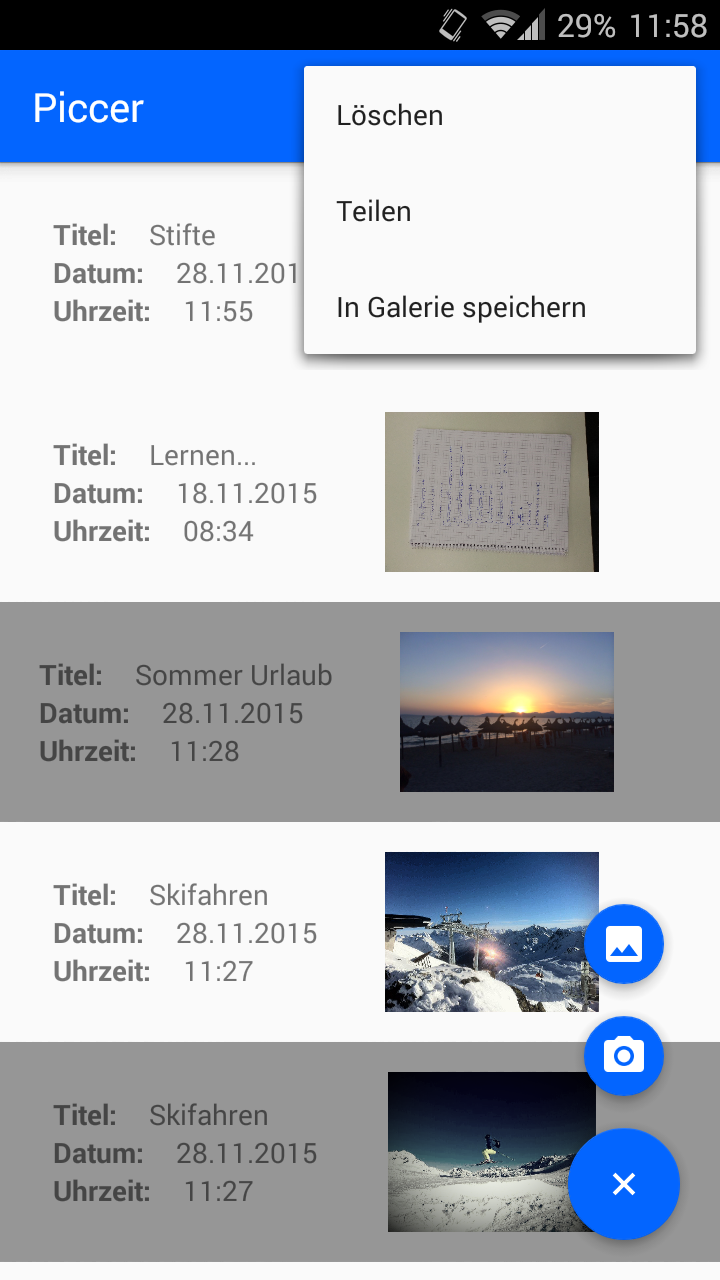
\includegraphics[width=120px]{../images/bild_3}
\caption{Mehrfachauswahl}
\end{wrapfigure} 


\begin{wrapfigure}{r}{0.3\textwidth}
\label{Bild4}
\begin{center}
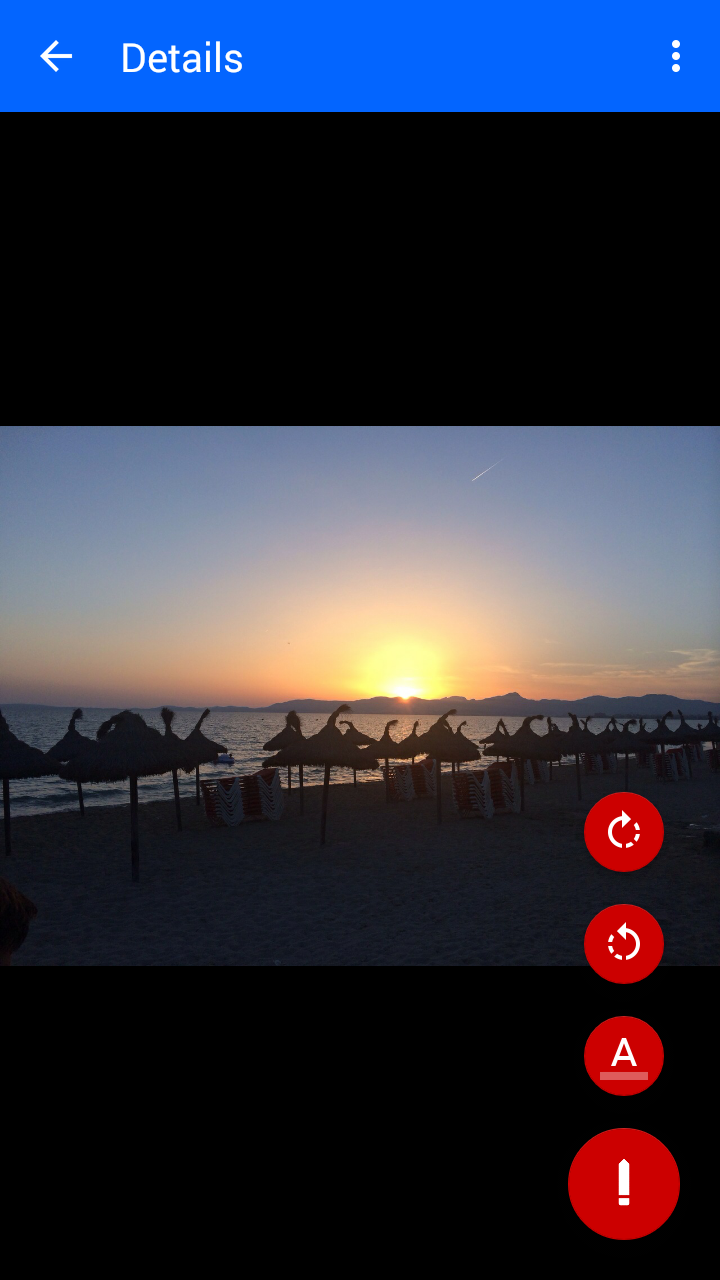
\includegraphics[width=120px]{../images/bild_4}
\end{center}

\caption{Detail Ansicht}
\end{wrapfigure}

